% 中文研究稿；基于 Elsevier CAS double-column v2.4，使用 XeLaTeX。
\documentclass[a4paper,fleqn]{cas-dc}
% Preserve CAS's STIX math encodings when ctex loads fontspec.
\PassOptionsToPackage{no-math}{fontspec}
\usepackage[UTF8,scheme=plain,fontset=fandol]{ctex}
\usepackage[numbers,sort&compress]{natbib}
\usepackage{booktabs,tabularx,multirow,array,amsmath,amssymb}
\usepackage{tikz}
\usetikzlibrary{arrows.meta,positioning}
\usepackage{pgfplots}
\pgfplotsset{compat=1.18}
\usepackage{enumitem}
\usepackage{balance}
\usepackage{lastpage}
\usepackage{microtype}
\usepackage{xurl}
\hypersetup{colorlinks=true,linkcolor=blue!45!black,citecolor=blue!45!black,urlcolor=blue!45!black}
\setlist[itemize]{leftmargin=1.4em,itemsep=1pt,topsep=3pt}
\setlength{\emergencystretch}{2em}
\renewcommand{\figurename}{图}
\renewcommand{\tablename}{表}
\renewcommand{\refname}{参考文献}
\newcommand{\localtablecaption}[1]{\refstepcounter{table}\par\raggedright\small\textbf{表~\thetable}\par#1\par\medskip}
\newcommand{\localfigurecaption}[1]{\refstepcounter{figure}\par\raggedright\small\textbf{图~\thefigure：}#1\par}
\newcommand{\skill}{\textit{Skill}}
\newcommand{\dataset}{\mathcal{D}}
\newcommand{\unknown}{\texttt{unknown}}
\newcommand{\methodname}{分层证据核验}
\ExplSyntaxOn
\cs_set:Npn \__first_footerline: { \footnotesize 中文研究稿（未投稿）\quad 2026-11-11 }
% CAS always prints an ORCID footnote, including when none was supplied.
\RenewDocumentCommand \printorcid {} {}
% Keep the official CAS layout; add stretch to its deliberately zero-width
% keyword overlay so a correctly placed overlay does not trigger an overfull box.
\RenewDocumentEnvironment { Abstract } { o }
{
  \group_begin:
  \IfNoValueTF { #1 } {} { \tex_gdef:D \abstractname { #1 } }
  \parindent 0pt
  \box_if_empty:NTF \g_stm_key_box
    { \leftskip = .35\textwidth }
    {
      \dim_gset:Nn \l_tmpa_dim { \box_ht:N \g_stm_key_box + \box_dp:N \g_stm_key_box }
      \leftskip .35\textwidth
      \hspace*{-.35\textwidth}
      \noindent\hbox_to_wd:nn {0pt} {\box\g_stm_key_box\hss}
      \skip_vertical:n {-\l_tmpa_dim}
    }
  \noindent\abstractname\par
  \skip_vertical:n {-4pt}
  \noindent\rule{.65\textwidth}{.2pt}\par\footnotesize
  \ignorespaces\everypar{\parindent=1.5em}
}
{\par\group_end:}
\ExplSyntaxOff
\newcommand{\NormalPassRate}{9.58}
\newcommand{\CheckPassRate}{89.21}
\newcommand{\MeasurePassRate}{78.42}
\newcommand{\NewPromptTokens}{1,394,720}
\newcommand{\NewOutputTokens}{32,153}
\newcommand{\NewPeakCny}{3.0467}
\newcommand{\NewPeakUsd}{0.457000}

\begin{document}
\let\WriteBookmarks\relax
\def\floatpagepagefraction{1}
\def\textpagefraction{.01}
\shorttitle{技能质量判别与证据条件化网络优化}
\shortauthors{SkillNet 研究项目}
\title[mode=title]{开放技能的质量判别与证据条件化网络优化：\texorpdfstring{\\}{ }基于 SkillNet 的可执行受控研究}
\author{SkillNet 研究项目（匿名研究稿）}
\begin{abstract}
开放技能的文档评分、来源真实与实际可用性常被混同，网络相似度也不能替代完整任务成功。
本文基于SkillNet-demo实现两项方法：用版本、机械反证和独立产物回执进行技能判别，
以及用版本匹配、条件证据和预算内兼容路径优化技能网络。
判别器在600个构造案例的父配置留出中检出140/140个已知故障、40个无害对照无误报，
并通过288次自建程序输出区分三种满足登记套件与九种缺陷实现；200个自然包仍有199个证据不足。
网络实验使用四份UCI公开表派生的构造任务，18个自建算子、928次开发探测、128个主留出输入及十种策略。
三个预定预算档的平均完整成功率为70.83\%，原生元数据最短路径为12.50\%，
人工固定流程和全局证据风险路径均为66.67\%；对强对照的增量集中在最紧预算，宽预算成功数持平。
中预算下执行调用比人工流程少7.14\%，但加入取证后总调用开销更高。
版本变化揭示按ID沿用证据的缺陷，事后合并精度与版本压力时完整方法也只通过12/24。
另保留自然包审查、真实模型评价、300次文本产物和历史网络回放作为测量参照。
结果支持按版本与输入条件判别、按完整路径评价优化，同时以弃权、强基线、全成本与反例限定结论。
新增两方法零模型调用；当前成果不构成自然技能总体认证或大规模SkillNet普遍领先的证明。
\end{abstract}
\begin{keywords}
智能体技能 \sep 质量核验 \sep 能力边界 \sep 独立产物验收 \sep 技能网络 \sep 条件化效用
\end{keywords}
\maketitle
% CAS records the current page before flushing appendix floats. Use the
% last shipped page so float-only pages are included in the printed total.
\gdef\lastpage{\pageref*{LastPage}}
\hypersetup{pdfauthor={SkillNet 研究项目},pdfsubject={技能质量判别与网络路径优化的受控研究},pdfproducer={XeTeX / TeX Live 2026}}
\section{引言}
可复用技能将说明、脚本与资源组织为能力单元，技能网络再通过检索和编排连接任务。
但文档完整、模型评分高、节点更多或检索相似度高，均不足以推出指定任务能够完成。
本研究关注两个直接问题：怎样得到可核验的技能质量判断及能力边界；怎样利用这些证据让技能网络在明确预算内完成更多任务。
评判依据应是可回放反证、独立完整产物和资源开销，而不是网络规模或模型自报成功。

SkillNet将技能创建、评价与连接整合为网络框架\citep{P01}；
SkillCT提出静态、动态与人类辅助画像\citep{P43}；SkillLearnBench区分技能文本、轨迹与任务结果\citep{P44}。
SkillsBench与ASSAY强调执行对照和条件化效应\citep{P02,P03}，
路由及多样性研究进一步关注大候选池与互补选择\citep{P04,P05}。
因此本研究不以新增评分维度、规则数量或确定性工具本身作为算法创新。
实质问题是：哪些证据能支持哪种决定，何种组合在什么条件下产生可重复增量，何时强而简单的对照已足够。

在SkillNet-demo基础上，本文交付两个可运行成果。
第一项是证据约束技能判别器，将固定版本的资源、机械接口反证与可信产物回执连接，
输出需要修复、被测范围通过、证据不足和超出已测范围。
第二项是证据条件化路径方法ECP，在有AND前提和预算约束的技能网络中，按版本及输入条件匹配开发证据，
保留互补的完整路径，并在新任务上重新验收。
前者不把静态一致当作运行认证；后者不把开发成功当作未来成功保证。

论文回答三个可检验问题：
\begin{itemize}
\item RQ1：机械反证和行为回执能否区分具有相似高文档分的不同实现，已测能力边界如何表达？
\item RQ2：条件证据与兼容路径能否在相同候选、预算和执行器下，比原生最短路径、全局证据路径及人工固定流程完成更多任务？
\item RQ3：增量来自条件化、集合互补还是版本绑定，取证成本和未见压力如何限制结论？
\end{itemize}

主要实证为600例判别诊断、288次自建程序输出，以及公开数据派生的18节点网络执行。
网络开发使用两份数据，主留出使用另两份数据和128个构造任务；十种策略、三档预算及压力结果完整报告。
相对原生元数据路径，ECP得到明确条件收益；相对人工与全局风险路径，成功增量主要限于紧预算。
合并新数值精度与版本变化后出现12/24的失败边界，前期取证也使本批总调用开销高于人工流程。
这些正负结果共同界定当前成果，不能推广为1,881个自然SkillNet节点的普遍优化或领域质量认证。

作为研究动机与测量参照，论文同时保留200个自然包审查、381个接口干预、54次模型评价、
300次五臂文本产物及1,152条既见网络回放。
这些历史实验不与新留出混合计算样本，也没有在本轮新增付费调用。
可核验性来自公开实现、固定输入与反例，而非引用数量或模板的期刊外观。

\section{相关研究与方法定位}
\subsection{可复用技能与技能网络}
早期自主智能体通过可执行程序积累技能，Voyager 展示了技能库在持续探索中的复用作用\citep{P11}。
ReAct、Reflexion、Toolformer、ToolLLM、ToolkenGPT、LATM 与 HuggingGPT 分别从行动推理、反馈、工具学习及任务分解等角度改进能力调用\citep{P12,P13,P14,P15,P16,P17,P18}。
这些工作支持将技能视为可复用的行为资源，但工具可被调用与工具在具体任务上有效仍是不同问题。
现代开放技能生态进一步使说明文档与资源包本身成为评价对象。
SkillNet、SkillCT 与 SkillLearnBench 是本文的近邻工作；本文不把多维度、能力边界或分层评价视为首创\citep{P01,P43,P44}。

SkillsBench 强调固定环境、有无技能对照及独立任务验收\citep{P02}。
ASSAY 通过干预估计任务条件下的技能效应，提示一个全局好坏分数不能替代条件化贡献\citep{P03}。
SkillRouter 研究大规模候选路由，DSR 研究相关性与集合多样性的联合选择\citep{P04,P05}。
其中重排中的 quality 是相关性权重，不能被解释为技能安全性或内在可信度。
本文的前五检索对照采用词法表示，ECP使用开发产物证据与显式前提；均不是这些训练模型的完整复现。

\subsection{评审、证据与风险控制}
G-Eval、MT-Bench 与 Prometheus 2 提供了结构化模型评审方法\citep{P24,P25,P26}，
JudgeBench 与位置偏差研究则表明，评审稳定性和表面一致仍需要客观参照\citep{P27,P28}。
ALCE、FActScore 和 RARR 将事实拆分、来源支持与修订联系起来\citep{P39,P40,P41}。
本文借鉴其证据思想，但将“文件与行号真实”“语义支持成立”“产物正确”作为三个不同测量层次。
引用可定位只解决第一层，不继承另外两层的准确性。

开放技能中的风险还包括恶意指令和正常功能受损。
生态实证、AgentDojo、InjecAgent 与 ToolEmu 提供了攻击与正常任务联合评测的依据\citep{P09,P10,P29,P30,P31}。
本文不执行恶意技能代码，也不由静态线索推断恶意。
共形风险控制与风险控制预测集合为错误放行约束提供了统计工具\citep{P36,P37}；
但当前数据的来源集中、独立校准标签缺失，不满足可直接宣称分布无关保证的条件。

\subsection{更新与系统优化}
DSPy、TextGrad、AFlow、ADAS 和 GEPA 表明，结构化反馈、候选搜索与程序优化可以改进系统配置\citep{P19,P20,P21,P22,P23}。
Skill++、COBRA-Skills 与 SkillHEX 将元数据演化、预算分配和失败修补用于技能生态\citep{P06,P07,P08}。
这类方法的效果仍应由独立任务和回归评测决定。
DPP 提供集合选择的标准工具，LinUCB 为预算内探索提供条件化决策视角\citep{P38,P42}。
SWE-bench、AgentBench、ToolSandbox 与 $\tau$-bench 则强调不同任务环境下的验收与行为轨迹\citep{P32,P33,P34,P35}。
本文的增量定位为：在固定包版本上连接可反驳声明、独立产物判别、条件证据与完整兼容路径，
同时披露该连接尚未获得的外部效度。

\section{分层证据核验方法}
\subsection{对象、声明和允许的结论}
把一个被评价对象写为
\begin{equation}
x=(s_v,q,m,a,e,b),
\end{equation}
其中 $s_v$ 是固定版本的技能包，$q$ 为任务，$m$ 为模型，$a$ 为执行器，
$e$ 为依赖和权限环境，$b$ 为上下文、时间及费用预算。
质量分不是只由技能名称决定的常量。
对每条能力声明 $c$，保存其输入、输出、前提、排除项、来源及版本，
再按表\ref{tab:states}记录当前证据状态。
来源哈希和行号有效说明该窗口可以被回放；它们不自动证明窗口支持声明，
更不证明相应行为在当前环境中成功。

\begin{table}[t]
\caption{证据状态及其允许支持的判断。状态不是从低到高可相加的质量等级。}
\label{tab:states}
\centering\small
\begin{tabularx}{\columnwidth}{p{.24\columnwidth}X}
\toprule
状态 & 允许的解释 \\
\midrule
仅声明 & 包或模型声称具备某能力，尚未得到验证。\\
静态支持 & 在登记资源和支持的分析范围内与声明一致。\\
发现冲突 & 有版本绑定的反证；需确认整体影响。\\
产物已验收 & 在指定任务、模型、执行器及预算下通过独立验收。\\
未知 & 缺材料、超出支持范围或尚未运行，不能补成零分或安全。\\
\bottomrule
\end{tabularx}
\end{table}

现有八维锚点包括契约一致性、完整性、静态可执行性、验证质量、维护性、
来源许可、成本意识和安全说明质量。
这些维度描述可观察材料；风险门禁、任务适配和真实效用另行测量。
纯咨询技能没有脚本，不因此被判为低质量。
反之，即使一个包的文档维度很高，也不能用其平均值抵消已发现的实质接口冲突。

\subsection{完整包与静态契约}
先核对资源清单、来源提交、字节数和 SHA-256，再分析受支持文本。
脚本只经语法树解析，绝不导入或执行社区代码。
本轮契约检查限于单一字面 argparse 解析器，支持选项存在性、必填、枚举值、
简单数值类型和布尔开关。
动态解析器、子命令、复杂位置参数和无法可靠解析的示例返回未知。
这种受限性使判断可反驳，也要求同时报告未知比例，而不能只报告命中案例。

对于受支持命令，构造已知错误和无害变换，比较只查参数名的基线、扩展契约检查及
按白名单声明重建的标准库 argparse。
后两者的约束逻辑不同，但共享语法树提取与词法预处理，不能被视为完全独立的端到端真值系统。
缺陷变体用于验证该机械契约，不充当整个技能的质量标签。

\subsection{来源绑定与语义支持分离}
模型返回的引用包含登记路径、源哈希、起止行、原文和支持或反证关系。
严格定位器只接受已提供的带编号材料，检查所有字段是否吻合。
随后，系统来源绑定器可以在冻结清单内额外取回资源，检查字节与哈希，并由系统抽取有界窗口。
模型不能利用引用路径读取清单之外的本机文件。

若模型只摘录了标注行的一部分，系统保留这种差异，不把重新抽取的完整窗口倒算成原模型正确。
若引用指向仅有目录登记的文件，后续补证单列为系统取证，不能说模型先前已经看过其正文。
绑定状态与语义支持状态使用独立字段，后者在未经审查时保持未评估。
这一设计借鉴事实与引用评价\citep{P39,P40,P41}，将版本绑定、定位、语义与结论覆盖拆开，
避免把一个可计算的引用有效率误用为综合质量准确率。

\begin{figure*}[t]
\centering
\begin{tikzpicture}[box/.style={draw=blue!45!black,rounded corners=2pt,fill=blue!3,align=center,minimum height=10mm,text width=34mm},>=Stealth,font=\small]
\node[box] (v) {固定版本与资源清单\\来源、字节、哈希};
\node[box,right=8mm of v] (c) {原子声明与静态反证\\接口、资源、前提};
\node[box,right=8mm of c] (b) {模型判断与来源绑定\\保留差异和未知};
\node[box,right=8mm of b] (o) {独立产物验收\\成功、失败及成本};
\draw[->] (v)--(c);\draw[->] (c)--(b);\draw[->] (b)--(o);
\node[draw,dashed,align=center,below=7mm of b,text width=70mm,minimum height=9mm] (u) {新实现：证据判别与条件化路径；仍待外部校准};
\draw[->,dashed] (o.south)|-(u.east);\draw[->,dashed] (u.west)-|(c.south);
\end{tikzpicture}
\caption{分层证据协议。实线为分层测量，虚线连接后文新增判别器与路径方法；外部效度仍待检验。来源绑定不替代语义判断；产物验收不等于跨任务的永久能力认证。}
\label{fig:protocol}
\end{figure*}

\subsection{独立产物验收与条件化效用}
对于任务 $q$ 的输出产物 $o$，令 $C_q$ 是预先定义的必需检查集合。
完整任务成功定义为
\begin{equation}
Y_q(o)=\prod_{k\in C_q}\mathbf{1}[k(o)=\mathrm{pass}],
\label{eq:success}
\end{equation}
而非各子检查通过比例的平均。
数值类型也属于契约，例如布尔真不能替代整数 1，浮点 8.0 不能替代要求的整数 8。
范围外或前提缺失的正确处置单独计量，不能与范围内的产物成功混成一个比例。

技能的任务条件化贡献为
\begin{equation}
\Delta_s=\frac{1}{H}\sum_{h=1}^{H}\frac{1}{|T_h|}
\sum_{t\in T_h}\bigl[Y_t(s)-Y_t(\varnothing)\bigr],
\label{eq:utility}
\end{equation}
其中 $h$ 为任务条件簇，$T_h$ 为该簇的输入与重复组合。
比较必须固定基础模型、必需任务说明、输出上限和可用工具，同时记录技能占用的上下文。
本文没有把无 Skill 组填充成无意义等长文本。
额外的无关技能组和仅操作契约组用于诊断上下文干扰及新增说明的贡献；
观测 token 不相等时如实披露，不宣称精确预算匹配。

经验能力边界是被测 $(q,m,a,e,b)$ 条件上的结果集合。
未观测到成功不证明数学意义的不可能，少数成功也不足以认证整个输入区间。
本研究不设未经校准的通用“90\% 即可自主使用”阈值，也不提出共形安全保证。

\subsection{技能网络的集合测量}
对任务 $q$ 的参考必要技能集 $G_q$ 与选择集 $S_q$，分别定义
\begin{align}
R@k(q)&=\frac{|G_q\cap S_q|}{|G_q|},\\
F(q)&=\mathbf{1}[G_q\subseteq S_q].
\end{align}
前者衡量平均参考覆盖，后者要求整组必要能力齐备。
二者都受参考标签遗漏等价技能的影响，并不是实际任务成功率。
将选择空间限制到固定前 20 个候选、固定取 5 个后，比较原顺序、MMR、DPP、
查询残差 DPP 和查询覆盖，检验“增加多样性总会更好”这一假设。
本文使用词法特征与名次相关性代理；没有继承 DSR 的训练编码器和原论文效果\citep{P05,P38}。

\subsection{成果一：证据约束的技能判别器}
\label{sec:decision-method}
在上述测量协议之上，实现可直接运行的确定性判别器，输入为包版本、资源清单、任务条件及登记行为回执。
它不是训练得到的神经分类模型，也不把八维文档均分直接转化为可用性。
判别按优先级执行：先检查登记资源缺失或哈希变化、入口语法和受支持的接口冲突；
再检查绑定相同包指纹、执行源码和输入指纹的可信行为回执。
外部提交的 \texttt{success=true} 或任意通过JSON不能自行成为回执。
只要存在已确认的机械反证或登记任务失败，输出“需要修复”；
没有反证但缺少足够行为材料，输出“证据不足”。
只有指定套件全部必需检查通过，才输出“被测范围内通过”；
请求一个未在回执中出现的新输入时，输出“超出已测范围”。

这里的能力边界是可核对的集合，而非从少数样本外推的输入区间。
令 $H_v$ 为版本指纹，$T_v$ 为登记的输入哈希集合，$O_v(h)$ 为独立验收结果。
对一个没有静态反证的版本，允许的通过结论为
\begin{equation}
\operatorname{pass}(v,h)\Rightarrow h\in T_v\ \land\ O_v(h)=1.
\end{equation}
套件通过只描述 $T_v$ 中的观察；即使整数求和实现已通过24个输入，新的
\texttt{[999]} 也不能直接得到同等认证。
该规则牺牲自动放行覆盖以保持结论与证据一致，故必须与检测率同时报告弃权和正确放行。
“无害静态例被保留为未知”不是误报，也不是成功认证。

相比纯文档评分，判别器能给出具体反证及其资源位置；相比只查参数名，
它额外覆盖必填、类型、枚举、文件完整性与语法；相比单纯静态过滤，
行为回执可区分相同接口下的正确与错误产物。
这些优势限于已实现规则和明确验收任务。
自然语言建议是否有帮助、领域知识是否正确、复杂脚本是否安全，仍缺少独立人类参照，不能据此判定。

\section{成果二：证据条件化的网络路径优化}
\label{sec:network-method}
\subsection{由节点分数转向有前提的完整路径}
网络优化的目标为预算内的完整任务产物，而不是把高分节点排在前面。
把节点 $s$ 写为 $(H_s,R_s,A_s,c_s)$，分别表示实现资源指纹、必要前提集合、
完成后新增的能力事实及上下文字节成本。
初始事实集为原始CSV存在，目标事实为指标已完成。
路径 $P=(s_1,\ldots,s_l)$ 必须满足
\begin{align}
R_{s_i}&\subseteq F_{i-1},&F_i&=F_{i-1}\cup A_{s_i},\\
\sum_{s\in P}c_s&\leq B,&l&\leq5.
\end{align}
例如，任务同时要求按键去重、排除跨分割主体和删除空分数时，顺序为先去重、再排除、再删空，
指标节点依赖这些必要事实全部成立。
复合节点可一次提供三个清洗效果。
因此逐个取高分的前五个节点可能重复同一能力并遗漏必要阶段；
“节点各自看起来好”与“存在兼容的完整路径”不是相同条件。

\subsection{证据匹配、条件分组与搜索目标}
本文实现 evidence-conditioned path（ECP）。证据只来自开发集的独立产物探测。
匹配键为完整工作资源的 SHA-256 与可观察条件组，而不是节点名称。
解析节点按是否含CSV引号分组，指标节点按是否存在阈值边界分组，其余按全部条件合并。
条件标记由任务适配器提供，所有策略均可见；它们不是验收答案，也尚未由通用语义识别器自动提取。

对匹配组中的成功数 $u_{s,g}$ 与探测数 $n_{s,g}$，定义排序启发量
\begin{equation}
\widetilde q(s,g)=\frac{u_{s,g}+1}{n_{s,g}+2}.
\end{equation}
将已观测到组内失败的节点排除，再枚举预算内的兼容路径，选择
\begin{equation}
\begin{aligned}
J(P)&=\sum_{s\in P}-\log\widetilde q(s,g)\\
&\quad+0.05\frac{\sum_{s\in P}c_s}{B}+0.02|P|,\\
\widehat P&=\arg\min_{P\ \mathrm{feasible}}J(P).
\end{aligned}
\label{eq:ecp}
\end{equation}
系数、分组、预算档位及比较规则在测试输出产生前固定。
未探测节点取先验 $1/2$，仍可能被选中；这明确是探索性路由，不是把未知标成可信。
各节点相关、前提状态可能变化，故 $\widetilde q$ 的乘积不是校准的路径成功概率。
式\ref{eq:ecp}只是小网络可穷举的确定性目标，不主张新的最短路径理论或普遍最优。

\subsection{与判别器的连接及公平对照}
成果一的通过状态严格绑定已测输入；成果二将开发观察用作选择新任务的假设，
仍须执行新路径并通过新的独立验收。
两者不可混为“已知输入通过，所以未来输入都被认证”。
每个新产物同时核对完整保留行、行序、计数、混淆矩阵及准确率、精确率、召回率、F1。
任一必要检查不合格均记失败；没有路径的弃权也按未完成计入分母。
全部策略共用验收器，其阻断错误产物的作用不能算成ECP独有的学习能力。

十种策略共用候选、任务、预算和执行器：词法、MMR及DPP前五后接原生规划器；
项目原生元数据最短路径；预先配置的正确人工流程；全局证据过滤后最短路径；
全局证据风险路径；ECP；条件证据前五后规划；去版本绑定的ECP。
全局风险路径与ECP仅区别于是否按输入条件匹配，去版本策略则故意只按ID沿用证据。
原生路径基线直接调用项目已有 \texttt{skillnet.frontier.plan}，没有另写较弱替代品。
人工流程使用预先选定的标准正确组件，是已知工作流条件下的强参照；
其人工配置成本未量化，因此不能直接当作可扩展自动路由器。
MMR/DPP使用词法表示，未复现训练版SkillRouter或DSR，不能宣称超过原论文模型。

\section{实验设计与复现约束}
\subsection{历史实验的数据范围与证据分母}
工程基线固定于提交 \texttt{0af2de6a}，总计 1,881 个对象，
包括 1,769 个社区原始包与 112 个项目派生卡片。
本轮完整包审查只使用开发集 D1 的 200 个原始包，其中 107 个来自
\texttt{sickn33/agentic-awesome-skills}，93 个来自 \texttt{alirezarezvani/claude-skills}。
资源登记共 1,441 个文件，其中 334 个 Python 文件；339 个不支持文本分析或二进制资源保留为不透明内容。
现有留出材料混有项目卡片，来源连接组也很少，因此本文不把开发实验写成独立外部测试。

表\ref{tab:inventory}汇总不同实验的测量单位。
同一任务在多种库规模、检索模式、提示或重复下出现，不会增加独立任务数量。
独立人类质量金标准仍为零；本文新增的自动真值只覆盖明确定义的构造任务。

\begin{table*}[t]
\caption{前期历史实验及其推断范围。两项新成果另见后文；规模不是可互换的独立样本数。}
\label{tab:inventory}\centering\small
\begin{tabularx}{\textwidth}{p{.18\textwidth}p{.28\textwidth}X}
\toprule
实验 & 实际规模 & 主要测量与限制 \\
\midrule
完整包静态审查 & 200 个 D1 原始包，470 条命令观察 & 静态一致、冲突、未知；不测运行成功。\\
受控接口干预 & 35 个父包，381 个命令变体 & 154 个已知机械缺陷、227 个原始或无害对照；不是整体质量标签。\\
模型评价先导 & 18 个训练父包，三臂共 54 次请求 & 评分结构、引用定位、未知覆盖；没有独立语义人审。\\
来源补证诊断 & 389 条引用，另取两个许可资源 & 只核对真实来源窗口，保留模型摘录差异。\\
新产物实验 & 30 个输入，五臂两次重复，共 300 次 & 24 个 CSV 输入、6 个边界输入；一个目标技能、受限文本执行器。\\
网络选择回放 & 192 份捕获，六策略共 1,152 条记录 & 32 个既见任务；不测真实编排执行。\\
\bottomrule
\end{tabularx}
\end{table*}

\subsection{静态干预与真实模型评价}
从静态一致且标准库重建参照也接受的命令中，每个父包按固定哈希顺序至多取三条，
得到 80 条命令、35 个父包。
错误干预包括虚构选项、遗漏必填、非法枚举和数值类型错误；
无害对照包括原命令、空白变化和可等价使用的等号形式。
按照父包而不是命令变体重采样，避免重复样本制造精确区间。

模型评价使用 D1 训练 20 例中的 18 例，其余两例在响应产生之前因打包字节上限排除。
普通 rubric、支持证据优先和反证优先三臂使用同一包材料及锚点，首臂位置循环平衡。
每个响应必须包含八个不同维度，未知或不适用不能同时给出数值。
该先导是同模型提示诊断，不是 SkillNet 或 SkillCT 完整评价流程的复现。

\subsection{新构造任务与独立验收}
新的五臂实验在首次请求前冻结输入、答案、代码指纹、预算及比较方向。
任务按 12 个构造条件组织：普通记录、含逗号字段、字段内换行、空字段、字面 NA 字符串、
纯空白字段、完整重复、仅键重复、7/8 天临界、闰年日期、未来及缺失日期、混合引号。
每种条件各生成 8 行和 48 行两个输入，共 24 个范围内案例。
另有缺输入、不可读输入、XLSX、图片、无读取权限和请求删除六个元数据边界案例。
这些边界案例没有测试实际文件解码或操作系统权限执行。

任务要求输出行数、逐列空值数、完整重复的多余行数、超过七天的记录数、最大已知年龄，
并保留输入标识与空操作列表。
只有解析后的空字符串计为空值，NA、null 字面值和空格不计为空；
重复与过期按原始记录逐条计数，不自动删改。
答案由生成器的记录结构与年龄变量构造，再分别经标准库 CSV/日期解析与 pandas 读取核对。
24 个 CSV 案例三路一致；六个边界标签由明确的优先规则规定。
正确参考产物、逐字段错误、错误数值类型和多余字段共 390 项诊断全部通过。
两个读取实现仍共享任务语义，这不等于独立领域专家验证。

五臂分别为无 Skill、原始包、原始包加证据操作契约、无关技能上下文、仅操作契约。
目标为固定版本的 \texttt{data-quality-auditor}；原始上下文包含主文档及
\texttt{data\_profiler.py} 文本。
补充契约指出原脚本的 uniqueness=90、timeliness=85 是默认值而非测量，
并要求以任务定义为准逐项计算。它没有修改或执行社区脚本。
无关上下文取自天气资源生命周期、Solidity 安全和组织文化三个 D1 技能，并在整行字节上限内截取。
其长度接近原始上下文，但没有精确匹配实际 token 数。

\subsection{已完成历史模型实验的顺序、成本与统计}
两组真实模型实验均直连 DeepSeek 官方 API，使用 \texttt{deepseek-flash}，
关闭思考，温度为零，单次输出上限 2,048 token。
文档当时标注 DeepSeek-V4.1-Flash-1017；API 返回的是可变别名，不能作为不可变权重证明。
新实验并发为二；每个任务--重复组合下循环轮换五臂顺序，不依据结果重试或换模型。
实际完成全部 300 次，无基础设施失败及未运行项。

费用使用实际返回用量乘官方峰时、未缓存输入单价计算保守上界，
分别控制在 5 美元和 20 元人民币以内；两种币种的口径不是汇率换算。
缺失用量或费用状态未知时停止继续调度，并保留已在途结果。
账户余额差不作为逐次独立账单。

范围内结果按条件簇聚合，比较原始包相对无 Skill、证据契约相对原始包、
仅契约相对无 Skill、证据契约相对仅契约、无关上下文相对无 Skill。
对 12 个条件均值做 10,000 次重采样，给出条件百分位区间和配对胜负平。
这些条件来自目的性构造，不是独立随机抽取的真实任务族；区间不表征社区技能总体，
也不用于多重比较下的显著性或等效性认证。

网络回放则固定两个库规模、BM25/Hybrid/Fabric 三种模式和既见的 20/12 个任务。
Fabric 捕获只含图扩展，不含 LLM 重排。
选择器不接收参考标签，固定词/汉字双字组 TF-IDF 和名次推导的相关性。
全部 12 个库--任务--模式组别及六策略均保存，避免只报告有利单元。

\subsection{判别器留出诊断与自建程序行为试验}
为检查新判别器，构造60个父配置，每个含10种版本，共600例；
按父配置固定40个开发、20个留出，留出200例含七类已知故障各20例、40个无害对照和20个不支持解析器例。
故障为未知参数、缺必填、非法枚举、错误类型、缺入口、资源变化和语法错误。
这些是研究者控制的机械干预，不是60个天然社区技能，也不是由独立专家给出的整体质量金标准。
对照含仅参数名、标准库argparse、文档均分阈值及去模块消融。
文档均分阈值0.8为本研究的工程适配，不能作为发表版SkillNet评价器的复现。

行为试验使用整数求和、稳定全行去重及DAG判定三个明确任务族，每族四种自建实现，共12个程序；
每个实现固定24个输入，共288次真实输出。
三种实现满足登记套件，九种实现植入可观测缺陷；所有文档都可取得约0.92的同类启发评分。
执行代码和输出回执均有字节指纹，验收器与被测实现分离。
这些观察验证“有相同高文档分的不同实现仍可由产物区分”，不估计自然技能优劣的发生率。

\subsection{公开数据派生的18节点可执行网络}
为从历史检索覆盖推进到真正路径执行，另建立一个可审计的18节点实验网络：
解析、按键去重、跨分割排除、空分数删除、指标计算及三阶段复合清洗各三个版本。
节点包括正确、条件受限和未探测实现；公开说明对同能力保持中性，ID为不透明散列。
选择接口只接收ID、能力、文本、资源指纹及字节成本，拒收测试答案、输出、实现键和缺陷标签。
不执行社区包；工作进程只允许本研究固定编写的算子。

原始表来自UCI：开发使用Iris（150行）和Wine（178行），留出使用WDBC（569行）与Banknote（1,372行）
\citep{UCIiris,UCIwine,UCIwdbc,UCIbanknote}。
各原始文件、下载归档、DOI、CC BY 4.0许可说明及指纹随稿保存。
将各文件第一数值特征归一化为四位小数分数、目标映射为二元标签，
再显式加入冲突重复、跨分割主体、空字段、含逗号及换行的引号字段和0.5阈值边界。
它们是\emph{公开数据派生的构造审计任务}，不代表原数据集分类准确率，不涉及临床判断。
八种清洗需求、24/72两个行数、两个引号条件及两个边界条件，形成每数据集64个任务。
开发128个、主留出128个，另从留出材料构造24个高精度数值压力输入。
任务语义和算子库跨数据集共享，故这种划分不是跨任务族或自然技能来源的独立验证。

独立参照按索引与自写CSV状态机读取，指标采用精确有理数；
worker使用标准库CSV、Decimal或各受测变体。
参照不导入规划器或worker实现；规划器也不导入答案计算和算子函数。
两路仍共享研究者规定的任务语义，降低实现耦合不等于第三方真值。
开发集共实际执行928次单节点探测，测试结果不可用于这些证据。
方案、输入、代码快照、公开元数据及基线在测试执行前冻结；这不是外部时间戳预注册，
研究者知道构造规则，不能称为独立双盲测试。

\subsection{预算、主估计量与压力检验}
预算为每任务元数据最低可行路径字节的1.0、1.5及2.0倍，向上取整，至多五次算子调用。
不使用测试成功来挑预算。
主估计量先在每个留出任务内平均三档二元成功，再平均128个任务；两个数据集权重相同。
32个清洗--引号--阈值条件块各有两个来源、两个行数，按块进行10,000次配对条件重采样。
这只描述所选构造条件的变动；不作真实任务总体置信度、多重比较显著性或分布无关保证。

固定压力包括新数值精度、取证后节点换版本以及缺失全部必要指标节点。
另做三次不透明ID置换，仅检验命名/并列顺序敏感性，复用相同输入。
主运行共7,856个策略决定，完全相同输入及实现路径共享一次执行，实际为1,204次路径执行、3,934次算子调用。
因此7,856不是独立任务数，1,204也不是全部不同输入。
在主结果产生后，再将精度与版本变化合并作明确标注的事后证伪：24个已有精度输入、240个决定、132次路径执行；
没有用该反例修改方法或计入预定主终点。
本轮新增方法与网络实验均为零模型调用、零API费用。
本机只在去凭据子进程运行自建代码；Linux CI另在无网络、只读、非root、去能力及限资源容器复现同批输入。
容器复现不是新增科学样本，也不是对社区恶意代码的安全认证。

\section{实验结果}
\subsection{成果一：可运行的质量判别与边界输出}
\label{sec:gate-results}
\begin{table}[t]
\caption{质量判别器的构造留出诊断。20个新父配置共200例；故障140、无害40、范围未知20。}\label{tab:gate}
\centering\small
\begin{tabularx}{\columnwidth}{Xrrr}
\toprule
方法 & 检出/140 & 误报/40 & 弃权 \\
\midrule
文档均分阈值适配 & 0 & 0 & 0 \\
仅参数名 & 20 & 0 & 60 \\
标准库 argparse & 80 & 0 & 60 \\
去接口检查 & 60 & 0 & 140 \\
去完整性检查 & 100 & 0 & 100 \\
完整判别器 & 140 & 0 & 60 \\
\bottomrule
\end{tabularx}
\par\vspace{3pt}\raggedright\footnotesize 阈值为本研究适配，不是发表版SkillNet的复现。完整判别器的60次弃权含40个缺行为证据的无害例；静态一致不自动获得可用认证。
\end{table}

在按父配置留出的200个构造案例中，完整判别器检出140/140个已知机械故障，
40个无害对照无误报，60例保持弃权（表\ref{tab:gate}）。
标准库argparse检出80/140；增加的60例来自缺资源、版本变化和语法规则，
不能写成“接口解析优于标准库”。
去接口检查降至60/140、去完整性检查为100/140，分别说明模块的有限增量。
文档阈值适配未检出这些干预，不能据此断言所有模型评分无效。

在288次自建程序行为试验中，完整判别器保留三种满足登记套件的实现，并为九种缺陷实现给出失败见证。
仅接口与文档路线仍会放行九种错误实现；只做静态门禁则12种都缺少可用性证据。
因此实际成果是能输出“修复、被测范围通过、证据不足、超出已测范围”的程序，
以及反证和输入边界，而不是一个没有依据的好坏平均分。
288次输出来自12个实现、每个24输入；不是288个自然技能。

同一判别器复核200个自然包，只对一个包给出三条已知参数冲突，其余199包仍为证据不足。
470条命令仍为134条静态一致、3条冲突、333条未知，包含79个无法解析入口的观察，未将其删除。
这说明自然包覆盖距离总体质量判定尚远。
构造留出全检出与自然包低覆盖应同时呈现，不能只挑前者报告100\%准确。

\subsection{成果二：完整产物收益与强对照}
\label{sec:network-results}
\begin{table*}[t]
\caption{18节点可执行网络的全部主留出结果。每档均为128个输入，弃权按未完成计；三档均值以同一128任务为单位。}\label{tab:network-main}
\centering\small
\begin{tabularx}{\textwidth}{Xrrrr}
\toprule
策略 & 1.0倍 & 1.5倍 & 2.0倍 & 三档均值(\%) \\
\midrule
词法前五＋路径 & 8 & 8 & 8 & 6.25 \\
MMR 前五＋路径 & 8 & 56 & 56 & 31.25 \\
DPP 前五＋路径 & 8 & 56 & 56 & 31.25 \\
原生元数据最短路径 & 16 & 16 & 16 & 12.50 \\
人工固定流程 & 0 & 128 & 128 & 66.67 \\
全局证据过滤＋最短路径 & 0 & 64 & 64 & 33.33 \\
全局证据风险路径 & 0 & 128 & 128 & 66.67 \\
ECP 完整方法 & 16 & 128 & 128 & 70.83 \\
条件证据前五＋路径 & 4 & 88 & 88 & 46.88 \\
ECP 去版本绑定 & 16 & 128 & 128 & 70.83 \\
\bottomrule
\end{tabularx}
\par\vspace{3pt}\raggedright\footnotesize 预算锚为只用元数据求得的最低可行路径字节数，非根据测试成功选取。上下文字节不是LLM token或费用。人工流程与全局风险路径在两档宽预算上均与完整方法持平。
\end{table*}

表\ref{tab:network-main}给出全部策略和三档预算。
ECP完整方法的主估计为70.83\%，原生元数据最短路径12.50\%，配对差58.33个百分点；
人工固定与全局证据风险路径均为66.67\%，差值仅4.17个百分点。
相对元数据基线有224个预算案例改善、0个恶化、160个持平；
相对人工/全局风险均为16个改善、0个恶化、368个持平。
这些都是128任务在三档预算上的重复比较，不能按384个独立输入解释。

中预算下ECP、人工固定与全局风险均完成128/128。
ECP相对这两个强对照的主终点增量全部来自最紧预算：16/128对0/128。
所以不能写成宽预算下求解能力超过已知正确流程。
全局过滤后最短路径在中预算仅64/128；这表明只过滤已知坏节点仍可能把未探测变体选成便宜路径。
条件证据前五仅88/128，完整路径为128/128，说明在本网络中先保留互补能力再求路径比逐节点截断有效。
词法、MMR和DPP的较低数值只适用于当前表示与小网络，不能作为对训练路由器的优越性证明。

\begin{table}[t]
\caption{ECP相对各对照的三档平均成功差（百分点）。32个构造条件块的10,000次条件重采样；不作总体或多重检验显著性主张。}\label{tab:network-effects}
\centering\small
\begin{tabularx}{\columnwidth}{Xrr}
\toprule
对照 & 平均差 & 95\%条件区间 \\
\midrule
词法前五＋路径 & 64.58 & [58.31, 70.83] \\
MMR 前五＋路径 & 39.58 & [28.12, 50.00] \\
DPP 前五＋路径 & 39.58 & [29.17, 50.00] \\
原生元数据最短路径 & 58.33 & [50.00, 64.58] \\
人工固定流程 & 4.17 & [1.04, 8.33] \\
全局证据过滤＋最短路径 & 37.50 & [27.08, 47.92] \\
全局证据风险路径 & 4.17 & [1.04, 8.33] \\
条件证据前五＋路径 & 23.96 & [13.54, 34.38] \\
ECP 去版本绑定 & 0.00 & [0.00, 0.00] \\
\bottomrule
\end{tabularx}
\end{table}

\begin{figure*}[t]
\centering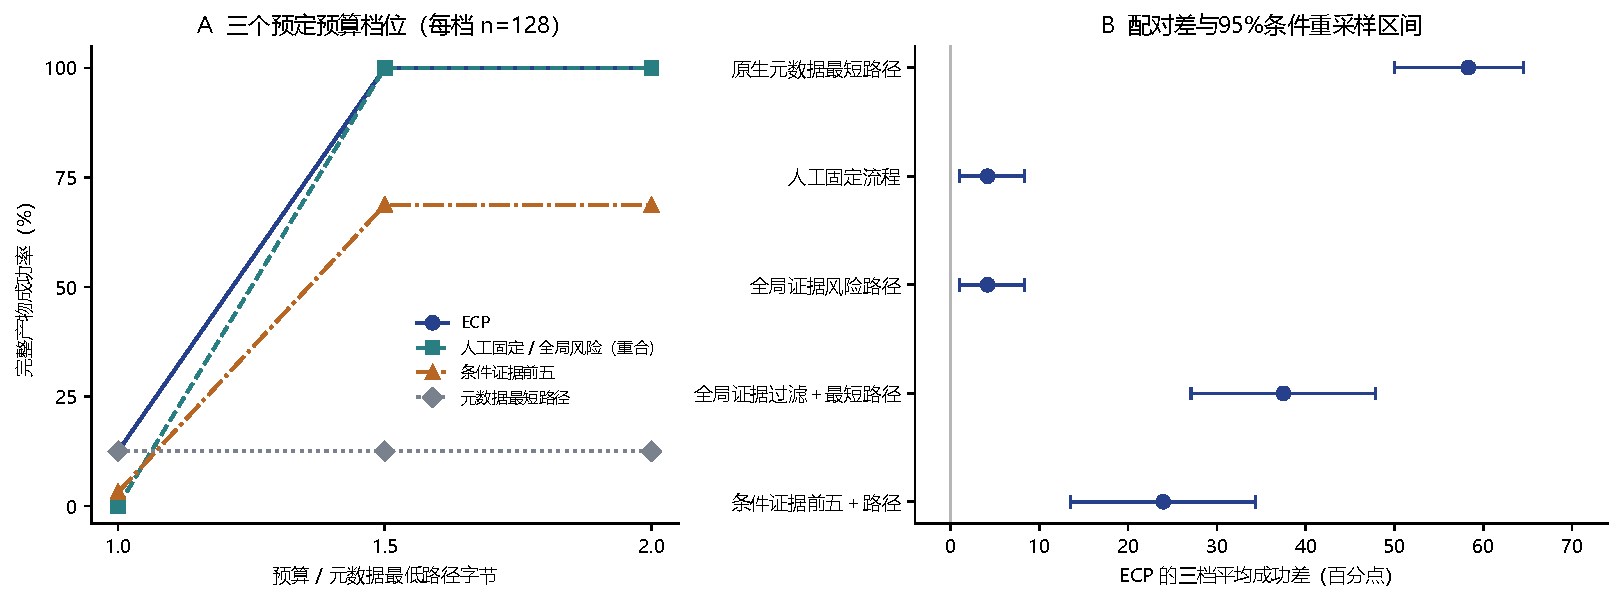
\includegraphics[width=.99\textwidth]{figures/network_budget_effects.pdf}
\caption{公开数据派生构造任务上的实际执行结果。左：预算不根据输出选取，点间连线仅辅助读图；人工固定与全局风险在三个主预算档重合。右：配对差的条件重采样区间，非标准误、非自然任务总体保证；颜色不编码显著性。}
\label{fig:network-budget}
\end{figure*}
表\ref{tab:network-effects}保留全部配对区间。
ECP相对元数据的95\%条件区间为[50.00,64.58]个百分点；
相对人工及全局风险均为[1.04,8.33]。
这描述当前32个构造条件块，不是已证实总体领先的概率。
两个留出数据集的每策略三档成功总数恰好相同（附表\ref{tab:network-datasets}），
说明受控语义和故障条件主导了差异，也限制了数据来源变化带来的外部效度。

\subsection{网络究竟改好了什么，成本是否值得}
\begin{table*}[t]
\caption{中预算资源与求解开销。包含失败尝试；前期取证为证据方法各自计入928次，非跨方法重复收费。}\label{tab:network-cost}
\centering\small
\begin{tabularx}{\textwidth}{Xrrrr}
\toprule
策略 & 成功/128 & 调用总数 & 上下文字节均值 & 含取证调用/成功 \\
\midrule
原生元数据最短路径 & 16 & 288 & 1801.5 & 18.00 \\
人工固定流程 & 128 & 448 & 2018.5 & 3.50 \\
全局证据过滤＋最短路径 & 64 & 448 & 1818.5 & 21.50 \\
全局证据风险路径 & 128 & 416 & 2023.5 & 10.50 \\
ECP 完整方法 & 128 & 416 & 1936.5 & 10.50 \\
\bottomrule
\end{tabularx}
\par\vspace{3pt}\raggedright\footnotesize 字节均值以启动路径为分母；本表五策略均启动128条。ECP含取证后为(416+928)/128=10.50，人工流程为448/128=3.50。调用不是货币成本。
\end{table*}

在同样完成128个中预算任务时，ECP用416次算子调用，人工流程448次，减少7.14\%；
平均上下文字节为1,936.5对2,018.5，减少4.06\%。
全局风险同为416次调用，但字节为2,023.5，ECP少4.30\%。
复合清洗与条件受限但适配的节点解释了这些变化；上下文字节仅是预先定义的资源代理，
复合节点按一次登记调用计，其内部三项操作未分别计价；
未实测CPU工作量、LLM token、端到端延迟或货币节省，不能替换成这些成本结论。

然而928次开发取证并非免费计算。
计入取证后，ECP本批为(416+928)/128=10.50次调用/正确产物，人工固定为3.50。
因此\emph{本批全成本不优于已知正确人工流程}。
若长期任务混合与版本稳定，按每任务节省0.25次调用粗略摊销，需约3,712个任务抵消探测调用；
这只是规划计算，未实测该规模，也没有计人工维护、探测异质成本和漂移后的重新取证。
方法是否值得采用，必须由新增覆盖、维护条件及完整成本决定。

\subsection{版本绑定的作用与不能组合的能力边界}
\begin{table*}[t]
\caption{固定压力实验及事后组合反例。各列均为中预算成功数。}\label{tab:network-stress}
\centering\small
\begin{tabularx}{\textwidth}{Xrrrr}
\toprule
策略 & 精度/24 & 换版本/128 & 缺能力/16 & 组合/24 \\
\midrule
词法前五＋路径 & 0 & 8 & 0 & 0 \\
MMR 前五＋路径 & 0 & 56 & 0 & 0 \\
DPP 前五＋路径 & 0 & 56 & 0 & 0 \\
原生元数据最短路径 & 0 & 16 & 0 & 0 \\
人工固定流程 & 24 & 64 & 0 & 12 \\
全局证据过滤＋最短路径 & 0 & 64 & 0 & 0 \\
全局证据风险路径 & 24 & 128 & 0 & 0 \\
ECP 完整方法 & 24 & 128 & 0 & 12 \\
条件证据前五＋路径 & 10 & 56 & 0 & 6 \\
ECP 去版本绑定 & 24 & 64 & 0 & 12 \\
\bottomrule
\end{tabularx}
\par\vspace{3pt}\raggedright\footnotesize 精度、换版本、缺能力在执行前固定；最右列为观察主结果后的证伪检查，复用同24个精度输入，不增加独立样本。组合条件中ECP只通过12/24，未据此调参。缺能力时全部方法弃权。
\end{table*}

替换已取证指标节点的代码但保留ID后，ECP与全局风险仍通过128/128，
仅按ID沿用旧证据的消融为64/128，人工固定也为64/128。
这支持资源版本匹配的必要性；因为全局风险同样成功，该收益不能全部归因于条件化。
去版本消融在无版本变化的主任务上与ECP完全一致，符合机制预期。

单独精度压力在中预算下，ECP、人工与全局风险均为24/24；最紧预算下ECP四次启动均失败。
进一步在观察主结果后合并精度与换版本，ECP只通过12/24，人工与去版本策略也为12/24，
全局风险为0/24（图\ref{fig:network-stress}）。
开发条件只区分是否存在0.5边界，没有编码任意小数精度；
无已知失败的候选也可能因浮点舍入失败。
这个反例说明单项压力通过不推出组合条件通过，平均组证据更不能变成整个输入族认证。
它作为事后证伪单列，未据此回调参数后冒充留出改进。

\begin{figure*}[t]
\centering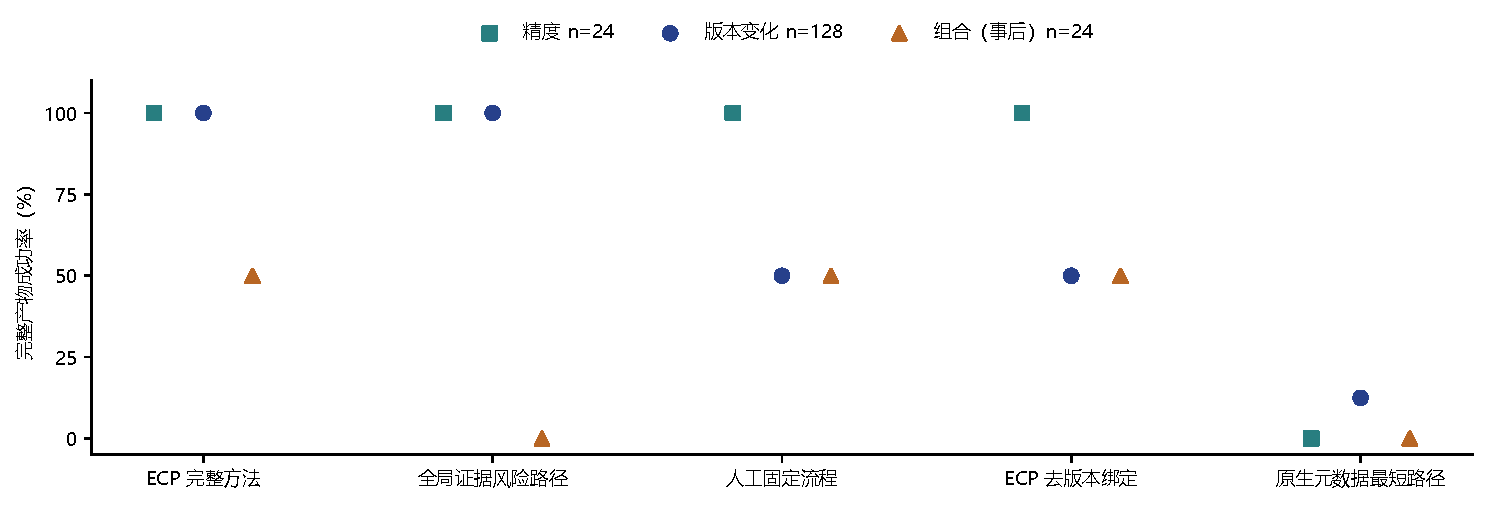
\includegraphics[width=.94\textwidth]{figures/network_stress.pdf}
\caption{中预算压力比较。不同列使用128或24个输入，各分母明确列出；组合压力为事后检查，复用24个精度输入。ECP单项均通过但组合只为50\%，是方法能力边界的实际反例。}
\label{fig:network-stress}
\end{figure*}
删除全部指标能力后，十种方法均弃权、成功均为零；这反映候选池上限，不是ECP特有优势。
三次ID置换后，ECP和全局风险均保持128/128、元数据16/128；MMR在40、16、24/128之间变化。
原始MMR为56/128，说明中性说明和并列顺序会影响词法截断。
置换仅为同输入敏感性检查，不能扩充主样本或证明任意命名下不变。

\subsection{静态检查发现了什么，又遗漏了什么}
470条实际命令观察中，134条在受支持范围内静态一致，3条存在接口冲突，
333条为未知，未知比例为70.85\%。
三条冲突来自同一 \texttt{senior-ml-engineer} 包的文档示例：
示例使用的参数没有出现在相应脚本的字面解析器中，而脚本要求的必填参数又未被提供。
这能反驳特定示例的一致性，不能据此判定整个包在任何任务上都无效。
41个父包的95次本地资源提及未能按当前规则解析，涉及84个父包--目标路径组合；
其中可能包含示例和可选阅读，不作为确认缺陷计数。

\begin{table}[t]
\caption{受控接口干预结果。强标准库参照与扩展规则均达到当前受限机械契约的满检出；不能外推成整体质量准确率。}\label{tab:faults}
\centering\small
\begin{tabularx}{\columnwidth}{Xrrr}
\toprule
已知缺陷 & 数量 & 参数名规则 & 扩展/标准库 \\
\midrule
虚构选项 & 80 & 80 & 80/80 \\
遗漏必填 & 22 & 0 & 22/22 \\
非法枚举 & 38 & 0 & 38/38 \\
数值类型 & 14 & 0 & 14/14 \\
合计 & 154 & 80 & 154/154 \\
\bottomrule
\end{tabularx}
\end{table}

表\ref{tab:faults}给出已知干预的结果。
只检查参数名会漏掉74个必填、枚举和类型错误。
扩展检查与标准库参照均检出154个构造错误，在227个原始或无害对照上均无误报。
按35个父包平均，扩展检查的检出差为38.14个百分点，
条件重采样区间为29.88--46.00个百分点。
这是受限机械缺陷的诊断增量，不是超过标准库的新算法，也不是通用技能质量准确率。

在事后代码结构审查中，两个数据与机器学习技能包的六个方法主体只返回字面
\texttt{success=True}，并带有实现占位注释。
它们不能独自证明所声明业务已经完成，但整个包是否有其他实现路径仍未实测。
早期扫描还曾把行尾解释性注释作为命令参数，增加了11条错误线索；
修正词法处理后，线索从14条降为3条。
修正前源码与数据均保留，说明核验器本身也必须接受反例和语境复核。

\subsection{高定位有效率没有构成质量准确率}
\begin{table}[t]
\caption{真实模型评价先导。引用分母只来自结构合格响应，定位有效不代表语义支持。}\label{tab:judge}
\centering\small
\begin{tabularx}{\columnwidth}{Xrrr}
\toprule
提示 & 结构合格 & 引用定位 & 未知维度 \\
\midrule
普通rubric & 17/18 & 123/125 & 9/136 \\
支持证据优先 & 18/18 & 132/135 & 9/144 \\
反证优先 & 18/18 & 127/129 & 15/144 \\
\bottomrule
\end{tabularx}
\end{table}

54次真实评价中，53次通过结构检查。
普通rubric有一个响应同时给出“未知”状态和分值1，按预先规则记为不合格，未自动补值。
合格响应的389条引用中，382条通过严格定位，比例98.20\%。
表\ref{tab:judge}中三种提示的定位有效率相近，反证优先输出更多未知和冲突，
但没有独立语义金标准，不能判其更准确。
结构不合格响应的引用不进入定位比例，分母明确保留。

七条未通过定位的引用逐条复核后，四条是没有完整复制标注行的摘录，
三条指向目录中存在、但未放入编号正文的许可文件。
它们不能统称为虚构证据。
事后来源绑定器为全部389条引用取得了真实窗口：386条来自已提供的编号文档，
另三条由系统额外取回两个登记许可资源。
四条模型摘录差异仍保留，额外取证的来源也单列。
这验证的是可追溯窗口，不是389个语义判断正确。

\subsection{历史文本产物实验：格式正确与计算正确明显分离}
\begin{table*}[t]
\caption{五臂实际产物结果。范围内每组48次；边界处置每组12次。费用只汇总范围内请求的峰价上界，不是独立账单。}\label{tab:execution}
\centering\small
\begin{tabularx}{\textwidth}{Xrrrrr}
\toprule
方法 & 合格数 & 成功率(\%) & 边界 & 平均输入token & 元上界 \\
\midrule
A0 无 Skill & 4/48 & 8.33 & 12/12 & 1706 & 0.2060 \\
A1 原始包 & 2/48 & 4.17 & 12/12 & 7122 & 0.7259 \\
A2 原包＋契约 & 4/48 & 8.33 & 12/12 & 7372 & 0.7500 \\
A3 无关上下文 & 6/48 & 12.50 & 12/12 & 5651 & 0.5847 \\
A4 仅契约 & 7/48 & 14.58 & 12/12 & 1955 & 0.2299 \\
\bottomrule
\end{tabularx}
\end{table*}

已完成的历史实验共300次请求，无基础设施错误、未运行或输出截断。
范围内五臂合计240份产物中只有23份完整通过，成功率为\NormalPassRate\%。
移除输入标识、哈希与额外字段等元数据约束后的数据指标合格数与主终点一致，
因此低成功率并非主要由形式字段导致。

表\ref{tab:execution}显示，原始包为2/48，无Skill和原包加契约均为4/48，
无关上下文为6/48，仅契约为7/48。
这些数值没有建立通用的优劣排序：只有一个目标技能，重复结果相关，输入是目的性构造，
无关上下文也没有精确匹配观测token。
特别地，无关上下文偶尔取得较高成功数，不能被解释为“不相关知识更好”，
而应提醒研究者避免从小样本排序直接推出方法胜负。

\begin{table*}[t]
\caption{预先固定的配对比较。差为百分点；区间是12个构造条件簇的条件重采样百分位区间，未经多重比较校正，不是总体保证。}\label{tab:effects}
\centering\small
\begin{tabularx}{\textwidth}{Xrrr}
\toprule
比较 & 均值差 & 95\%条件区间 & 胜/负/平 \\
\midrule
A1$-$A0 & -4.17 & [-14.58, 4.17] & 1/3/44 \\
A2$-$A1 & +4.17 & [-4.17, 12.50] & 3/1/44 \\
A4$-$A0 & +6.25 & [0.00, 12.50] & 3/0/45 \\
A2$-$A4 & -6.25 & [-12.50, 0.00] & 0/3/45 \\
A3$-$A0 & +4.17 & [0.00, 10.42] & 2/0/46 \\
\bottomrule
\end{tabularx}
\end{table*}

预先固定的条件簇比较见表\ref{tab:effects}。
原包加契约相对原始包的平均差为4.17个百分点，条件区间覆盖零；
仅契约相对无Skill的差为6.25个百分点，区间下界为零。
因此没有建立稳定的正向优势，更没有总体或跨模型保证。
仅契约的输入占用明显少于原始包，但它仍有41/48份范围内产物不合格，
不能仅凭较少token就认定已经得到可靠能力。

\begin{figure*}[t]
\centering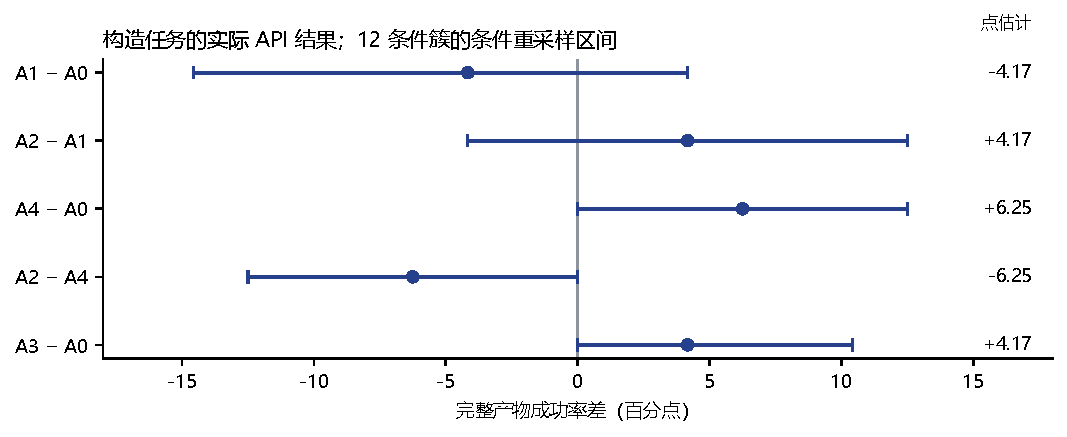
\includegraphics[width=.88\textwidth]{figures/paired_effects.pdf}
\caption{预先固定的五个配对比较。每个点来自实际API产物；线段为选定12个构造条件簇的95\%条件重采样区间，非标准误，也非技能总体的置信保证。图中颜色不编码显著性。}
\label{fig:effects}
\end{figure*}

\subsection{能力边界需要由失败层次刻画}
\begin{table}[t]
\caption{范围内输入规模分层。每个单元格为合格产物数/24次，两个重复不是独立任务。}\label{tab:sizes}
\centering\small
\begin{tabularx}{\columnwidth}{Xrr}
\toprule
方法 & 8行 & 48行 \\
\midrule
A0 无 Skill & 4/24 & 0/24 \\
A1 原始包 & 2/24 & 0/24 \\
A2 原包＋契约 & 4/24 & 0/24 \\
A3 无关上下文 & 6/24 & 0/24 \\
A4 仅契约 & 7/24 & 0/24 \\
\bottomrule
\end{tabularx}
\end{table}

六类明确元数据边界在五臂、两次重复下共60次处置全部合格。
与此同时，48行输入的120份范围内产物没有一份完整通过；
8行输入的120份产物只有23份合格（表\ref{tab:sizes}）。
边界处置和计算成功显然不能混成一个指标。
这些结果也不足以把8行认证为可靠能力区间，或把48行判定为绝对上限：
只观测了两个规模，且较小规模仍有较高失败率。

错误主要集中于过期记录计数：240份范围内产物中有216份在此项失败，
最大年龄错误20份、逐列空值错误10份、完整重复错误9份、行数错误4份。
这些错误计数可以重叠，不能相加后当作不同失败任务数。
即使温度为零，120个相同输入--方法的重复对中仍有7对的完整通过状态不同，
24对的产物数值不同；温度设定不是外部服务完全确定性的证明。

以一个8行普通CSV为例，基准日为2026-11-11，八条记录年龄依次为
$[7,1,31,8,31,7,1,0]$ 天，严格超过七天的记录应为3条。
同一输入的一次无Skill响应报告2条，原始包报告3条，而原包加契约报告0条。
其他字段可同时正确。
这一案例给出了可手工复核的失败机制，不能被引用定位或结构合格所弥补。

\subsection{事后测量诊断：平均检查掩盖完整任务失败}
这是在预定主分析之外进行的解释性诊断，不作为新的显著性检验。
每份范围内产物有9个输出字段及1个精确schema检查，共2,400项检查，
仅259项失败，平均检查通过率为\CheckPassRate\%。
即使只平均五个数据测量检查，通过率也有\MeasurePassRate\%，
但完整产物成功率仍仅\NormalPassRate\%。
该比例不是原项目既有质量分；它说明把多个容易条件与关键条件平均，
可以让同一批输出看起来远比实际可用程度好。

对同一批产物做发布门禁回放，全部接受会放行217份不合格产物；
全部拒绝虽无错误放行，但正确产物覆盖为零。
完整验收器门禁放行23份，按本构造真值没有错误放行。
后者是验收规则定义下的发布决定，不增加模型求解成功，也不是开放任务上的风险保证。
其价值在于显式呈现错误放行与覆盖，而非用全拒绝伪装优秀系统。

\subsection{网络侧：多样性没有自动形成完整能力覆盖}
\begin{table*}[t]
\caption{全库Fabric组的历史检索回放。既见12例不是新留出；相关性与完整集合覆盖分别计量。}\label{tab:routing}
\centering\small
\begin{tabularx}{\textwidth}{Xrrrr}
\toprule
方法 & 20例R@5 & 20例F & 既见12 R@5 & 既见12 F \\
\midrule
原顺序 & 80.00 & 55.00 & 78.47 & 58.33 \\
MMR .7 & 80.00 & 55.00 & 75.69 & 50.00 \\
原核DPP & 80.00 & 55.00 & 78.47 & 58.33 \\
残差DPP .5 & 80.00 & 55.00 & 78.47 & 58.33 \\
残差DPP 1 & 80.00 & 55.00 & 78.47 & 58.33 \\
查询覆盖 .5 & 80.83 & 55.00 & 78.47 & 50.00 \\
候选池上限 & 100.00 & 100.00 & 94.44 & 91.67 \\
\bottomrule
\end{tabularx}
\par\vspace{2pt}{\footnotesize R@5与F单位均为百分比；候选池上限使用参考标签作事后上界，不是实际选择器。}
\end{table*}

六种策略在全部192份捕获上产生1,152条选择记录。
表\ref{tab:routing}展示全库Fabric组，其余组别随数据一并提供。
基准20例中查询覆盖的平均召回从80.00\%升至80.83\%，
完整参考集合覆盖仍为55.00\%。
既见12例中，MMR的完整覆盖从58.33\%降至50.00\%，
查询覆盖也降至50.00\%；DPP类代理多数保持原结果。
这些结果不支持“增加多样性必然改善网络”的假设，也不能据此否定使用不同表示和训练模型的DSR。

基准20例的必要参考技能都在候选池中，但原前五只有55\%完整覆盖，
说明该组存在选择余地。
既见12例的池上限本身也不完整，未召回的参考能力无法靠重排补回。
由于任务均已使用、参考标签按技能名匹配且可能遗漏等价技能，
本文不把这组指标宣称为新的外部泛化或实际编排成功率。

\section{讨论与有效性威胁}
\subsection{可信性来自可反驳性及独立测量}
质量判别器对明确规则输出资源级反证，对行为输出独立检查结果，且版本和输入指纹可复核。
相比只给文档平均分，它能解释缺陷在哪里，以及哪些请求仍未覆盖。
对照、模块消融、保留失败与未知、冻结选择后再执行，降低了循环论证和只报告有利案例的风险。
网络参照采用与worker不同的CSV读取和精确算术路线，重放还能核对每个选择及产物。
这些提高的是本设计的内部可核验性，不等于独立领域专家已认可语义金标准。

评价的权威性不能由大模型品牌、引用顶刊数量或双栏模板替代。
本文未建立自然技能的整体好坏标签、人类仲裁一致性或外部基准排名；
不能报告通用质量准确率、语义支持准确率、恶意代码检出率或校准风险上界。
构造故障全检出与自然200包中199包证据不足必须同时保留。
一旦独立验收器遗漏了任务要求，系统仍会出错，故验收器也需要新的反例和外部审查。

\subsection{两个成果各自解决了什么}
成果一给出可使用的判断机制：有机械或行为反证则请求修复，指定输入全部通过才限定放行，无证据或越界则弃权。
它在自建任务中区分了同类高文档分的正确和错误实现；对咨询型自然技能仍不能提供普遍判定。
新增规则与标准库互补，并非所有部分都比现有简单工具更强。

成果二将同一证据用于版本匹配、条件适配和完整路径选择。
相对无质量证据的元数据最短路径，完整产物成功明显增加；
相对逐节点前五截断，AND前提与复合能力保留避免了部分能力缺口。
但已知人工流程和全局风险路径在宽预算下已经完成全部主任务，完整方法没有在这些条件下进一步提高成功数。
版本压力收益也被全局风险路径取得，不能只归于条件分组。
本文没有学到通用路由器，也没有比较已训练的SkillRouter或DSR模型。

本批ECP需要928次探测；只报告执行阶段7.14\%调用节省会误导采用决定。
对已知而稳定的流程，人工预配置在当前批次更省总调用。
网络探索只有在未知配置、多条件复用、维护漂移或紧预算新增覆盖的收益抵消取证成本时才可能值得。
目前没有长期运行、真实token与计费、节点维护时间或端到端延迟数据，不能宣称已实现实际部署降本。

\subsection{有限条件证据无法认证整个任务族}
ECP的平滑频率是排序启发量，不是概率校准成果。
节点错误可相关，上游输出分布会改变下游条件；微小的条件分组无法表达所有输入属性。
主任务成功和单项压力成功都没有阻止组合压力的失败。
这支持在新任务上继续验收和有条件弃权，不支持“开发组无失败即可长期自主执行”。
成果一对未见输入返回越界，成果二则探索新路径；二者的结论强度不同，应在产品中分别显示。

18节点为研究者编写，缺陷和任务也是研究者安排，可能使方法有利于已知的条件特征。
四份UCI数据提供公开可追溯输入，但清洗语义、故障和算子跨源共享；两个留出数据集结果完全相同尤其提示模板主导。
这不是对原始1881对象网络的自然端到端改进证明，更不能当作临床或原始分类任务性能。
任务标记由可信适配器给出，自动识别和审计这些标记的成本未测。
小网络穷举没有证明在千级异构网络上的可扩展性。

\subsection{历史实验为何仍保留}
模型引用的高定位有效率只证明来源窗口可追踪，没有建立语义正确性。
300次文本产物的23/240范围内成功，揭示平均逐项通过与完整可用之间的测量差距；
工具受限条件未允许社区脚本运行，故不能推出原技能在正常工具环境下同样失败。
原包加契约和历史自然网络重排没有稳定收益，这些负结果不能被新受控网络成功覆盖或改写。
54及300次请求来自可变服务别名，同一任务重复、多个策略和预算都不是独立样本。
全部条件区间均只对目的性设计作描述，不承担总体显著性或共形风险保证。

\subsection{尚需完成的外部验证}
下一阶段应以独立领域人员的盲标与仲裁检验真实语义质量，公开仲裁前一致性；
将自然技能接入合格隔离执行环境，使用未参与方法设计的真实任务和新的独立验收；
再比较发表实现、同材料模型评审、确定性工具、人工流程及ECP，计入取证和维护的完整成本。
应预先固定来源分组、输入族、预算和重要最小效应，保留拒绝与失败，而不按观察结果选择最有利任务。
此路线是扩大效度的后续任务，不属于本文已达成的结论。

\section{结论}
本文在SkillNet-demo上实现并检验了两项可运行成果：证据约束技能判别器，以及证据条件化的网络路径优化。
前者将可反驳的资源/接口证据与独立产物回执连接，输出修复、被测范围通过、证据不足和越界，
在构造留出诊断检出140/140个已知机械故障，并在288次自建程序输出上区分正确与缺陷实现。
自然包低覆盖同时表明，它尚不是通用技能质量认证模型。

后者在18节点公开数据派生任务网络中，把版本匹配、条件证据与完整兼容路径结合，
主留出三档平均成功70.83\%，高于原生元数据路径12.50\%；
对人工及全局风险路径仅提高4.17个百分点，宽预算成功数持平。
版本匹配降低了沿用旧代码证据的失败，完整路径减少了逐节点截断的能力缺口。
但前期取证使本批总调用成本高于人工流程，组合压力下只通过12/24。
因此成果是具有明确反例和适用条件的可复现方法及数据，而非对自然SkillNet网络普遍领先的主张。

\section*{数据、代码与研究状态声明}
工程与审查入口为\url{https://github.com/qing1989620/skillnet-demo}研究分支及
\url{https://github.com/qing1989620/skillnet-demo/pull/2}。
随稿包保存双栏LaTeX、44篇定向阅读论文及4份数据引用、全部新方法源码、冻结数据、协议与代码快照、
逐次选择/输出、分析和出图脚本、离线复现命令、旧产物数据与必要第三方许可。
新方法复现不读取模型密钥，不需要付费API；已有54及300次模型实验仅从记录重算，不重新收费执行。
原始UCI文件按CC BY 4.0归属说明随包保存，改造过程明确记载；社区完整第三方材料和密钥不进入稿件包。

本文为学位研究及导师审阅准备的中文研究稿，未投稿，未经独立同行评审。
采用Elsevier CAS双栏模板只表示版式来源，不表示期刊录用或官方认证。
44篇文献为方法、实验和局限的定向学习，不宣称全部属于SCI顶刊、逐字通读或系统性元分析。
代码、分析和写作使用AI辅助，模型输出是研究对象，不是独立人类评审者。
正式学位提交或投稿前，需由研究负责人核对作者、机构、研究规范与目标格式。

\bibliographystyle{cas-model2-names}
\bibliography{references,datasets}
\clearpage
\appendix
\section{逐次结果与复现补充}
图\ref{fig:matrix}显示全部48个范围内输入--重复单元在五臂的二元结果。
每四行对应一个构造条件，包含两个输入规模及两次重复；灰色不合格项没有被删除或最佳重试替换。
逐次JSON记录还保留失败字段、实际输入输出token和响应指纹。

\begin{figure*}[t]
\centering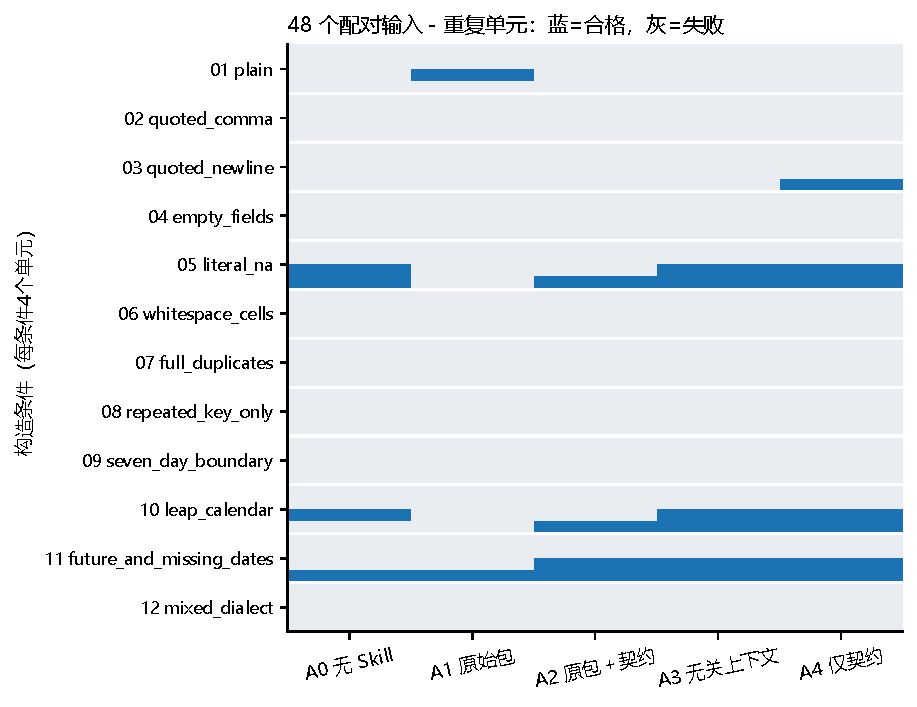
\includegraphics[width=.8\textwidth]{figures/artifact_matrix.pdf}
\caption{240份范围内实际产物的完整二元结果矩阵。数据为构造输入上的真实API输出；蓝色表示所有必需检查通过，灰色表示至少一项失败。条件排列在生成时固定，不按结果排序。}
\label{fig:matrix}
\end{figure*}

\subsection{输入与验收规则}
每个CSV包含 \texttt{id}、\texttt{amount}、\texttt{observed\_at}、\texttt{note} 四列。
构造输入的随机种子为20261111；闰年条件的基准日为2024-03-02，其余为2026-11-11。
原始记录的年龄变量保留于参考构造过程，序列化后经两个读取实现重新计算。
输入哈希由任务适配器提供供执行器复制，不把生成SHA-256作为能力测试。
每次请求是独立会话；执行器不会获得预期计数、验收代码或其他臂的答案。

对非完成状态，五个数据指标必须为空、操作列表为空，且状态须符合任务前提。
对完成状态，额外字段、缺字段、错误数值类型或任一错误指标均使完整任务失败。
这使正确格式、正确处置与正确测量分别可解释，同时防止全拒绝取得表面优胜。

\newpage
\subsection{代码与排版的验证}
新增构造任务及预算守卫通过专项检查，旧研究数据和源码指纹保留。
前期真实评价后曾修正跨平台类型标注，原始执行源码单独保存在代码快照中，
修正前后可执行语法树相同，未重复计入模型请求。
本文使用Elsevier CAS双栏类2.4和中文排版支持，由用户指定的TeX Live 2026中的XeLaTeX编译。
该模板提供版式，不代表目标期刊适配、录用状态或研究结论的权威性。

\subsection{不应从本文推出的结论}
不能将154个机械缺陷全检出写成所有技能100\%准确；
不能将来源窗口全部绑定写成语义判断全部正确；
不能将60次明确边界处置正确写成操作系统或真实二进制格式安全；
不能将观察成功数最高的方法写成跨技能、跨模型最优；
也不能将检索覆盖写成实际编排成功率。
这些限制是测量对象的一部分，而不是在结果产生后删去失败的理由。

\subsection{新网络的逐源与逐任务核对}
\begin{figure*}[p]
\begin{minipage}[t]{.48\textwidth}\vspace{0pt}
\localtablecaption{主结果分数据集核对。每格为同64个输入在三档预算下的成功总数/192。两个数据集的模式完全相同，反映构造语义主导的限制。}\label{tab:network-datasets}
\centering\small
\begin{tabularx}{\columnwidth}{Xrr}
\toprule
策略 & WDBC & Banknote \\
\midrule
词法前五＋路径 & 12/192 & 12/192 \\
MMR 前五＋路径 & 60/192 & 60/192 \\
DPP 前五＋路径 & 60/192 & 60/192 \\
原生元数据最短路径 & 24/192 & 24/192 \\
人工固定流程 & 128/192 & 128/192 \\
全局证据过滤＋最短路径 & 64/192 & 64/192 \\
全局证据风险路径 & 128/192 & 128/192 \\
ECP 完整方法 & 136/192 & 136/192 \\
条件证据前五＋路径 & 90/192 & 90/192 \\
ECP 去版本绑定 & 136/192 & 136/192 \\
\bottomrule
\end{tabularx}

\vspace{8mm}\raggedright\small
主留出只包含128个不同输入，每个数据集64个。表中192为64个输入乘三档预算；两个数据集同样的成功总数不代表192个独立任务，也不能用重复预算缩窄区间。

\medskip
原始记录位置：\texttt{research/skill\_network/results/} 下的 \texttt{prepared-v3}、\texttt{calibration-v2}、\texttt{execution-v2}、\texttt{analysis-v1} 和 \texttt{joint-posthoc-v1}。
公开元数据、执行前选择、worker请求、原始输出和逐项判定分别保存，便于审查是否发生答案泄漏或失败删除。

\medskip
完整复现同时检查原始源文件指纹、开发/留出隔离、逐次选择、全部产物、三档聚合、条件重采样及事后反例。CI复现报告记录了无凭据、无网络及只读边界；它增加实现可移植性证据，不增加科学样本或领域认可。
\end{minipage}\hfill
\begin{minipage}[t]{.48\textwidth}\vspace{0pt}
\centering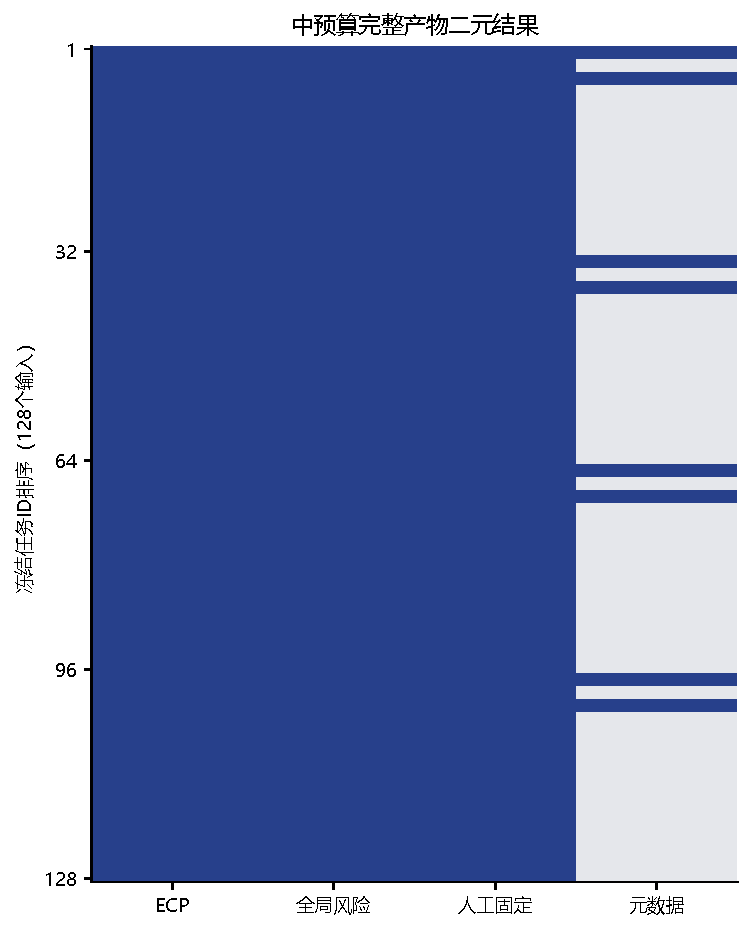
\includegraphics[width=.96\linewidth]{figures/network_binary_matrix.pdf}
\localfigurecaption{中预算128个主输入的二元完整成功矩阵。按冻结ID排序，蓝色为全部检查通过，灰色为失败或弃权；这里只显示四个预定代表策略，全部十策略记录随稿。}
\label{fig:network-matrix}
\end{minipage}
\end{figure*}

新网络的协议、代码快照和选择记录先于worker执行写出；原始冻结目录中的准备/校准路径名只标识历史运行，不作为外部预注册证明。
离线复现逐条重算7,856个主运行选择、240个事后选择和全部独立验收，再用同一随机种子重算区间。
可选重执行合并928次开发探测、1,204条主路径及132条事后路径共2,264个worker请求，不增加独立样本。

\end{document}
